%------------------------------------------------------------
%
\documentclass{llncs}%
\usepackage{quotes}
\usepackage{epstopdf}
\usepackage{bsymb}
\usepackage{alltt}
\usepackage{amsmath}%
\usepackage{graphicx}
\usepackage{hyperref}
\usepackage{enumitem}
\usepackage{amssymb,amsfonts,textcomp}
\usepackage{color}
%-------------------------------------------
\begin{document}
%
\title{Configuring Code Generated from Event-B}

\author{A. Edmunds~\inst{1}, K. Wiederaenders~\inst{2} and K. Reichl~\inst{2}}

\institute{University of Southampton, UK\\
\and Thales Transportation Systems, Germany
}

% Templates
% Interface
\maketitle
%
\begin{abstract}
The Event-B method, and  its tools, provide a way to formally model systems. Tasking Event-B is an extension facilitating code generation from Event-B.  We have recently begun to explore the issue of re-usability, of generated code. In this work describe two features , interface generation and templates. To improve re-usability, we extract an interface from an Event-B model of the environment, and provide automatically generated simulation code. The provision of the interface allowed further experimentation with hand-crafted code. In a second enhancement to the approach, we introduce a method of using templates, for code generation. We avoid hard-coding code common to particular target; we add the common code to template and introduce tags for template expansion or code injection. Template expansion allows copying of code verbatim, and generator-tags allow code injection linked to custom code generators. This is an extensible approach, making use of the Eclipse extension-point mechanism. This approach can be applied to any text output, and was used in the FMI C code generator, fro which we take our examples. 
 \end{abstract}
%
%
\section{Overview}
%
Rodin is a  tool platform~\cite{abrial10rodin} for the rigorous specification of critical systems, using the Event-B approach~\cite{ABR10}. The tool was developed in the RODIN project~\cite{RodinTool}, and experience with industry was gained in the DEPLOY project~\cite{DEPLOY}. Tasking Event-B~\cite{Edmunds2009,Edmunds2008,ae2011a,ae2012b} is an extension to Event-B that facilitates generation of source code; code generators are currently available for Java~\cite{JavaSpec}, Ada~\cite{ada2005}, C for OpenMP~\cite{openmp}, and C for FMI~\cite{FMISTD}. The work reported here has been funded by the ADVANCE project~\cite{advance}, a continuation of the Event-B research effort, this time focussing on co-simulation of Cyber-Physical Systems. But, the initial discussion and some of the ideas for the work reported here, arose from an industrial collaboration with Thales Transportation Systems, Germany; during which time we undertook a case study, involving a top-to-bottom appraisal of the Event-B approach - from abstract specification to implementation. One of the main issues of concern was that of re-use of generated artefacts. Until now the deploy-time issues of target configuration, and how to tailor the generated code for re-use has not been addressed. 

It is certainly mainstream engineering practise to re-use artefacts, wherever possible. This provides benefits in terms of time and cost savings, and improved reliability. In programming terms re-use of code often involves the use of patterns, sub-classing, and use of polymorphism. In the work that we report here, we too have aimed to improve re-use in this way. We first discussed this as future work, in~\cite{ae2011a}, where we alluded to the fact that a generated environment simulation may be replaced by one that interfaces with the `actual' drivers of the target system. In Sect.~\ref{interfaces} we introduce interface generation, from Tasking Event-B, and present two short examples of how the interfaces can be used in the development process.

Often when a system is being implemented, there is a large amount of code that is common to the particular target implementation, perhaps for system life-cycle management, or system health monitoring. But, this code is independent of the actual state and behaviour of the part of the system being formally modelled. We have provided a simple extension to allow the use of templates; with an injection mechanism to allow insertion of  such `boilerplate' code (copied verbatim), and also insertion of model-specific, generated, code.  The use of templates in the code generation approach should facilitate re-use of existing code, and importantly avoid having to hard-code such details. It will also provide a focal point for application of many configuration details, whilst at the same time permitting insertion of generated code at locations specified by the template writer. The tags that define insertion points, are linked to pre-configured code fragment-generators. We discuss this feature in Sect.~\ref{templates}. It should also be noted that the approach is suitable for use with any textual source and target file. In our work with FMI code-generation we developed, and made use of the template-based generator; but it was our aim to make the template mark-up, and code fragment-generators, both customizable, extensible and suitable for use with other text based input and output.  
%
\section{Event-B }
%
Event-B and Tasking Event-B
%
IL1 and protected Objects
%
\section{The Use of Generated Environment Interfaces}\label{interfaces}
%
%
The case study
%
%
%
\section{Templates: for Configuration and Re-use}\label{templates}
%
The Functional Mock-Up Interface~\cite{FMISTD} is a C-based interface that has been devised to facilitate re-use of simulation models. The re-usable components, known as Functional Mock-up Units (FMUs) implement the FMI API, and allows modular composition where FMU slave simulators are imported into a custom master simulation coordinator. The ADVANCE project~\cite{advance} is providing a way to co-simulate discrete Event-B models with continuous models of the environment. We have also developed a code generation approach where discrete, Event-B controller models can be translated into C code, for use in FMU simulation of discrete implementations. The FMUs can then be used for simulation and testing, with models of its continuous environment. We were able to re-use much of the generator code from the existing OpenMP generator, and just provide a new FMU-C specific generator.  

When generating code from Tasking Event-B, we found that there was a large amount of boiler-plate code, from the FMI API, that we did not want to hard-code. We thought that this provided a good opportunity to explore the use of templates in code generation. The templates provide an opportunity to re-use this `boiler-plate' code. It is also easily customised, so this is where we can make use of it for system configuration. In the first instance we surveyed the existing technology, such as Java Emitter Templates (JET)~\cite{JET}. We found that this provided a very expressive solution, but was unnecessarily complex for our simple needs. We provide an architectural overview in the diagram of Fig.~\ref{fig:templates}.
%
\begin{figure}
\centering
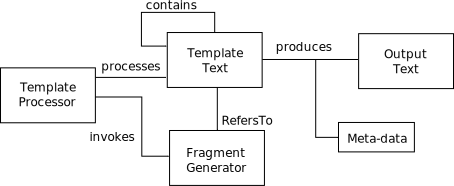
\includegraphics[width=0.8\textwidth]{templateOverview.png}
\caption{Overview of Template Use}
\label{fig:templates}
\end{figure}
%
\subsection{A Template Example}
In this diagram we can see that we have a number of artefacts involved in template processing; we have text-based templates, code-fragment generators, text output, meta-data output and a template-processor that does the work. The templates may contain plain-text (which is copied verbatim to the target during processing) and tags. The tags may refer to other templates, or code-fragment generators. The code-fragment generators are hard-coded generators that relate to certain aspects of the final output. By way of example, the code FMI code generator has a fragment generator that inserts the variable initialisations into the template we can see its use in~\ref{fig:templateExample}. 
%
\begin{figure}
\begin{center}
\begin{minipage}{0.8\textwidth}
//\#\# $<$addToHeader$>$\\
fmiStatus fmiInitializeSlave(fmiComponent c,\\
\hspace*{0.2cm}fmiReal relativeTolerance, fmiReal tStart,\\
\hspace*{0.2cm}fmiBoolean stopTimeDefined, fmiReal tStop)\{\\
\hspace*{0.4cm}fmi\_Component* mc = c;\\
\hspace*{0.4cm}//\#\# $<$initialisationsList$>$\\
\hspace*{0.4cm}//\#\# $<$stateMachineProgramCounterIni$>$\\
\hspace*{0.4cm}return fmiOK;\\
\}
\end{minipage}
\end{center}
\caption{An Example Template}
\label{fig:templateExample}
\end{figure}
%
%
The template is part of an implementation of the FMI API's \emph{fmiInitializeSlave} function. This is part of the `boiler-plate' C code for an implementation of an FMI slave, and the code in the example is common to all initialization functions. The first parameter of the function is the \emph{fmiComponent}, it is the `instance' of the FMU that is to be initialised; the other parameters relate to the simulation life-cycle.  However, an FMU also keeps track of state-variables which will be different for each model. These state-variables correspond exactly to the variables of the system that have been modelled in Event-B. As part of the code generation approach we generate an intermediate-language model ( the IL1 model). The fragment-generator can use the IL1 model, in the translation to the C source code.  In the template, we a placeholder (which we call a \emph{tag}), where we want the variable initialisation to occur. The tags in our example begin with the character string, //\#\#.  This string is customizable, since we have provided an extension point, for users to define which characters to use as tags. This makes use of the Eclipse extension mechanism. The string we chose allows the tag to be treated as a comment; so, that the remainder of the code can be syntax checked if required. This line is continued with $<$\emph{identifier}$>$ where an \emph{identifier} is supplied. A tag is usually (but not always) an insertion point; its \emph{identifier} can relate to another template (to be expanded in-line); or the name of a fragment-generator. The fragment-generator is a Java class that can be used to generate code; or meta-data that is stored for later use, in the code generation process  (see Fig.~\ref{fig:templates}). In the example we have three tags. We will show how the template processor uses the \emph{intialisationList} tag, as a code injection point to add variable initialisations, in subsection~\ref{injection}. The first tag \emph{addToHeader} identifies a generator that creates meta-data, this used at a later stage for generation of a header file. The last tag is not used in our example, since we have no state-machine diagrams in the model. But, if we did have state-machines in the FMU, we generate code to implement its initial state, in this location.
%
\subsection{Template Tags and Generators}
It is possible to categorize the users of Rodin into several types of users. One such type are the `ordinary' modellers, using Event-B in smaller organisations. But for large scale use one may have meta-modellers (to develop product lines for instance), another user may instantiate models (of the product line), a third is a system administrator/programmer that provides tool for the others. The extension points that we provide allows the system administrator/programmer to provide template utilities for the other users. The first extension point \\ \emph{org.eventb.codegen.templates.tag} has been provided to allow them to specify the \emph{tagCommentCharacters}. The second, \emph{org.eventb.codegen.templates.generator} has been provided to allow them to add new \emph{tag identifiers}, and \emph{GeneratorClass}es that implement \emph{IGenerator}. The \emph{IGenerator} interface defines a single \emph{generate} method which takes an instance of \emph{IGeneratorData} as a parameter. The \emph{IGeneratorData}  is a container for  a \emph{List} of objects, used by the \emph{generate} method, when generating the code fragment. The template-processor stores the link between \emph{tag identifier} and \emph{GeneratorClass} in a \emph{GeneratorMap} (repository). By adding a new \emph{tag identifier} and providing a new generator implementation, a Rodin-user (working at the implementation-level) has this new feature available for insertion into the template, to produce some specific output. 

\subsection{Code Injection} \label{injection}
We now return to our explanation of how the \emph{initialisationList} is processed, and refer back to the example shown in Fig.~\ref{fig:templateExample}. The template-processor scans each line, and copies the output; or inserts new text, or meta-data as required, until we reach the line with the \emph{initialisationList}. The template-processor finds the \emph{initialisationList} in the \emph{GeneratorMap}. It is linked to the \emph{InitialisationListGenerator} class, by the map. The class's \emph{generate} method is invoked, to begin the process of text insertion. A fragment of the \emph{InitialisationListGenerator} class can be seen in Fig.~\ref{fig:genCode}. The class defines variables that are used to hold the data retrieved from the \emph{IGeneratorData} object;  \emph{prot} and \emph{tm} are objects that are required to process the initialisations. In this case, the declarations are retrieved from the (IL1) \emph{Protected} object, and translated in turn.   
%
%
\begin{figure}
\centering
\begin{minipage}{0.85\textwidth}
\textbf{public class} InitialisationsListGenerator \textbf{implements} IGenerator \{\\
\hspace*{0.2cm}\textbf{public} List$<$String$>$ generate(IGeneratorData data)\{\\
\hspace*{0.4cm}List$<$String$>$ outCode = \textbf{new} ArrayList$<$String$>$();\\
\hspace*{0.4cm}Protected prot = null;\\
\hspace*{0.4cm}IL1TranslationManager tm = null;\\
\hspace*{0.4cm}\emph{//(1) Un-pack the GeneratorData}\\
\hspace*{0.4cm}List$<$Object$>$ dataList = data.getDataList();\\
\hspace*{0.4cm}\textbf{for} (Object obj : dataList) \{\\
\hspace*{0.6cm}\textbf{if} (obj instanceof Protected) \{prot = (Protected) obj;	\}\\
\hspace*{0.6cm}\textbf{else if}(obj instanceof IL1TranslationManager)\{\\
\hspace*{0.8cm}tm = (IL1TranslationManager) obj;\}\}\\
\hspace*{0.2cm}\ldots\\
\hspace*{0.2cm}\emph{//(2) Get the Declarations}\\
\hspace*{0.2cm}EList$<$Declaration$>$ declList = prot.getDecls();\\
\hspace*{0.2cm}\emph{//(3) Process each Variable Declaration/Initialisation}\\
\hspace*{0.2cm}\textbf{for} (Declaration decl : declList) \{\\
\hspace*{0.4cm}\ldots\\
\hspace*{0.4cm}String initialisation = FMUTranslator.updateFieldVariableName(\ldots);\\
\hspace*{0.4cm}outCode.add(initialisation);\\
\hspace*{0.2cm}\}\\
\hspace*{0.2cm}\emph{// (4) return the new fragment}\\
\hspace*{0.2cm}\textbf{return} outCode;\}\}
\end{minipage}
\caption{An Example Fragment-Generator}
\label{fig:genCode}
\end{figure}
%
%

The main steps are highlighted using numbered comments in the code. In step 1, the data is un-packed; in step 2, the declarations are obtained from the \emph{Protected} object; in step 3, the initialisation are translated, and add to an array of initialisation statements; in step 4, the initialisations are returned to the template-processor. The code that is generated is shown in Fig.~\ref{fig:codeOut}. 
%
\begin{figure}
\centering
\begin{minipage}{0.9\textwidth}
fmiStatus fmiInitializeSlave(fmiComponent c, fmiReal relativeTolerance,\\
\hspace*{0.6cm}fmiReal tStart, fmiBoolean stopTimeDefined, fmiReal tStop) \{\\
\hspace*{0.2cm}fmi\_Component* mc = c;\\
\hspace*{0.2cm}\emph{// (1) Injected By InitialisationsListGenerator $>>>$ }\\
\hspace*{0.2cm}mc-$>$i[c\_level\_controllerImpl\_] = 100;\\
\hspace*{0.2cm}mc-$>$b[c\_pumpOnReq\_controllerImpl\_] = fmiFalse;\\
\hspace*{0.2cm}mc-$>$b[c\_pumpOnCmd\_controllerImpl\_] = fmiFalse;\\
\hspace*{0.2cm}\ldots\\
\hspace*{0.2cm}\emph{// (2) $<<<$ End of Injection}\\
\hspace*{0.2cm}\textbf{return} fmiOK;\\
\}
\end{minipage}
\caption{The fmiInitializeSlave Function with Injected Code}
\label{fig:codeOut}
\end{figure}

In the generated code of Fig.~\ref{fig:codeOut} we see that variable initialisations such as,

\begin{minipage}{\textwidth}
\centering
mc-$>$i[c\_level\_controllerImpl\_] = 100;
\end{minipage}
have been generated, between the comments numbered (1) and (2). This initialisation seen here is very specific to the FMU approach. The FMI component \emph{mc} identifies an FMU; its integer variables are stored in an array \emph{i}[], and a variable named \emph{c\_level\_controllerImpl}, is accessed using an index into the array \emph{c\_level\_controllerImpl\_}. This is rather complex but should demonstrate the point that we can inject code of some complexity.

%
\section{Conclusions}
Tags for Template Expansion

Tags for Code Insertion with fragment generators

Tags for processing meta-data

Re-use of boiler-plate code, avoids hard-coding too.

Provided configuration, either manually through changing the template code, or by making use of tags as insertion points, that can make use of configuration data.
%
\bibliographystyle{plain}
\bibliography{MyBibTex}
%
%
%
\end{document}
